\documentclass[journal]{IEEEtran}

\usepackage[T1]{fontenc}  
\usepackage[utf8]{inputenc}  
\usepackage[portuguese]{babel}
\usepackage{graphicx}
\usepackage{subfigure}
\usepackage{enumerate}
\usepackage{ae}
\usepackage{color}
\usepackage{epstopdf}


\hyphenation{op-tical net-works semi-conduc-tor}

\begin{document}

\title{Introdução ao Processamento de Imagens}

\author{Victória Goularte - 12/0137691}

\markboth{Universidade de Brasília - UnB}
{Shell \MakeLowercase{\textit{et al.}}: Bare Demo of IEEEtran.cls for IEEE Journals}

\maketitle

\begin{abstract}
No trabalho são aplicadas operações consideradas de médio nível no processamento digital de imagens. São as operações morfológicas, de segmanetação e codificação de vídeo.
\end{abstract}

\section{Introdução}

\IEEEPARstart{A}{baixo} uma breve explicação sobre cada operação trabalhada:

\subsection{Morfologia}
A Morfologia Matemática em processamento de imagens trata de  extração de regiões de uma imagem, representação e descrição das formas de uma determinada região.

Este processo é considerado de nível médio onde a saída do
processo é um atributo da imagem.

Porém, como estes atributos atributos são resultados de processamentos na estrutura geométrica dos objetos. São representados em formato de imagens digitais

\subsection{Segmentação de imagens}
Tecnicamente a segmentação é subdividir uma
imagem em regiões ou componentes.

No sistema visual humano a segmentação é uma
tarefa subjetiva realizada no cérebro, pelos
neurônios entre as áreas corticais de nível alto
e médio.
A segmentação deve concluir quando os objetos
(ou regiões) de interesse para uma
determinada aplicação tenham sido isolados.

O método morfológico de segmentação utilizado nesse trabalho foi o de 'wathershed' que realiza a segmentação da imagem através do crescimento de regiões.

É definido como de fato um divisor de águas de uma imagem em níveis de cinza e é análoga à noção de uma bacia de captação de um heightmap. Em suma, uma gota de água seguindo o gradiente de uma imagem flui ao longo de um caminho para alcançar finalmente um mínimo local. Intuitivamente, o divisor de águas correspondem aos limites das bacias hidrográficas adjacentes das gotas de água.

\subsection{Codificação de vídeo}
Essa operação foi utilizada para estimar o movimento entre frames de um vídeo para obter o melhor preditor dentro de sistema DPCM. A técnica de obter o quadro formado a partir dos preditores é chamada de compensação de movimento.

\section{Metodologia}
O trabalho foi dividido em três partes(3 questões), que serão tratadas separadamente a seguir:\newline

\subsection*{Parte I}
Dada a imagem:

\begin{figure}[!htb]
	\centering
	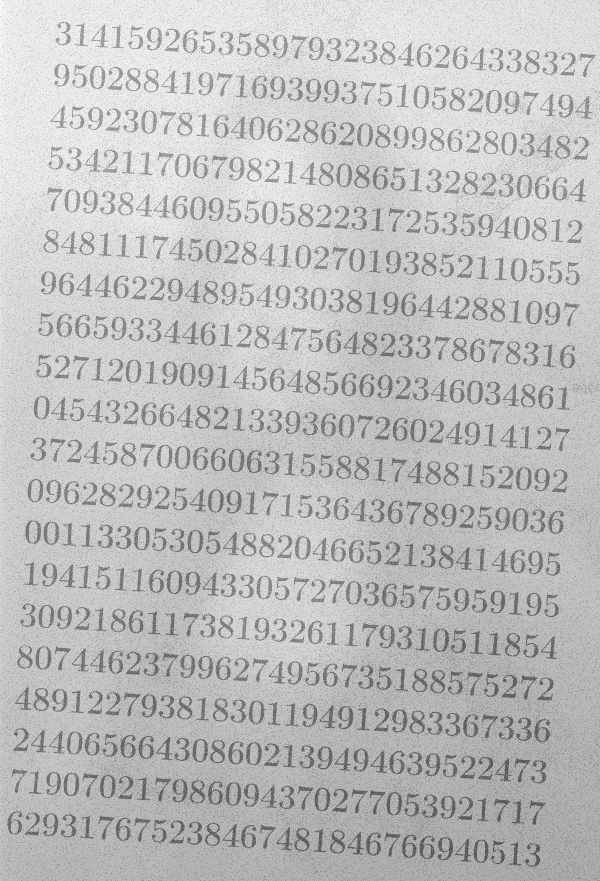
\includegraphics[scale=0.2]{morf_test.png}
	\caption{Original}
	\label{Original}
\end{figure}
	
Utilizando o MATLAB, um programa foi feito para que a imagem acima apresentada fosse modificada e resultasse em uma imagem binária com os objetos que a compõem pretos e fundo branco. Para isso, antes de qualquer coisa, a imagem foi binarizada e percebido que em certos pontos perdia-se informações, pois em alguns lugares o fundo e objetos estavam classificados em um mesmo nível de cinza fazendo com que objetos também se tornassem fundo. Então, fez-se a transformada bottom-hat que é é utilizada para realçar objetos escuros sobre fundo claro utilizando uma função do próprio MATLAB e alternativamente aplicando o fechamento na imagem obtendo apenas o seu fundo e depois subtraindo a fundo da imagem original, que também caracteriza uma operação bottom-hat, e os resultados obtidos foram:

\begin{figure}[h]
\centering
\subfigure[Imagem Bottom-Hat\_int]{
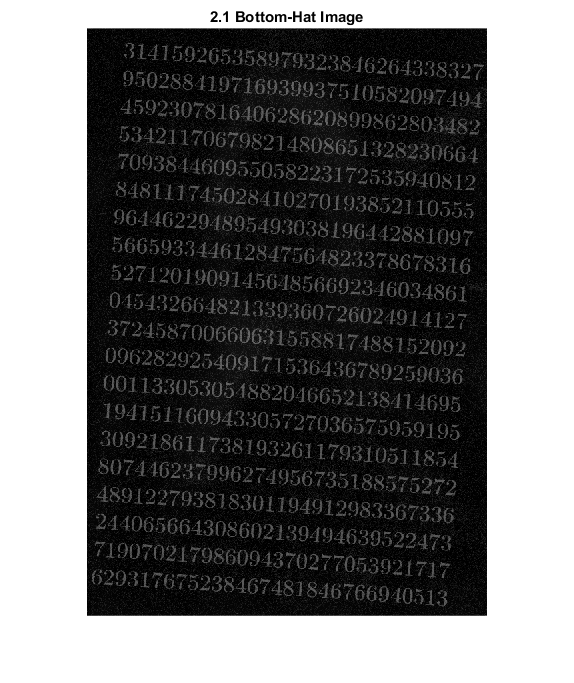
\includegraphics[scale=0.25]{q1-bh1.png}}
\subfigure[Fundo - Imagem\label{red2}]{
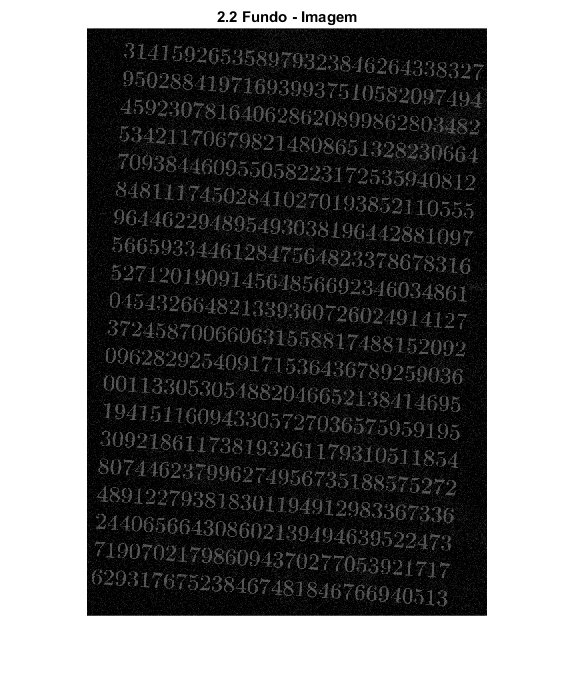
\includegraphics[scale=0.25]{q1-bh2.png}}
\end{figure}

Nota-se que o objeto se destaca melhor na bottom-hat feito obtendo-se o fundo e posteriormente subtraindo esse fundo da imagem origina. Então, sobre essa imagem foi aplicada a operção de identidade inversa para que os objetos ficassem pretos e fundo branco.

\begin{figure}[!htb]
	\centering
	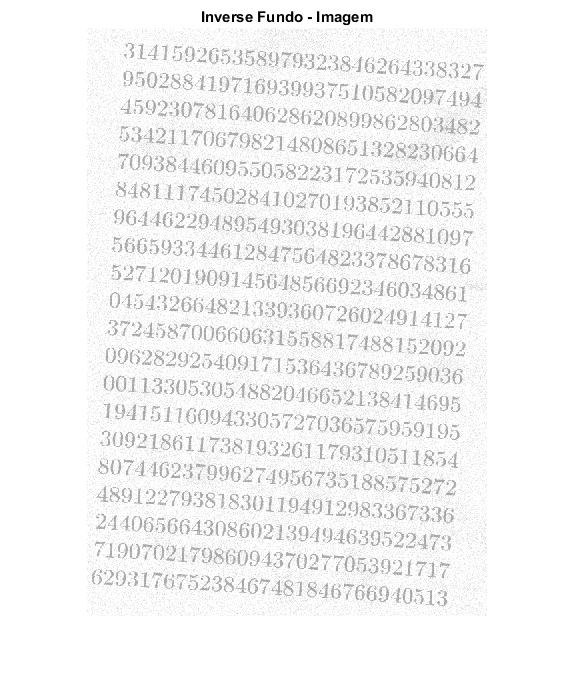
\includegraphics[scale=0.25]{q1-bh2-i.png}
	\caption{Inverse bottom-hat}
	\label{Original}
\end{figure}

Essa imagem foi binarizada para então destacar os objetos.

\begin{figure}[!htb]
	\centering
	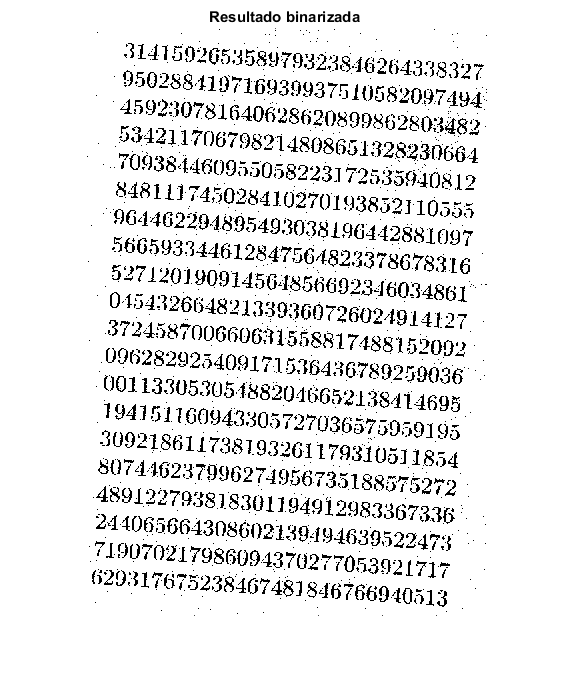
\includegraphics[scale=0.25]{q1-bh2-bin.png}
	\caption{Bottom-hat binarizada}
	\label{Original}
\end{figure}

Foram então percebidos falhas de preenchimento dos dígitos e certos ruídos na imagem, e para que melhorasse essa imagem foram aplicados outra operação morfológica de dilatação para completar os objetos em que havia falhas e um filtro de média para retirada dos ruídos. Por fim, ainda foi feito um fechamento para separar dígitos que se emendaram na dilatação

\begin{figure}[!htb]
	\centering
	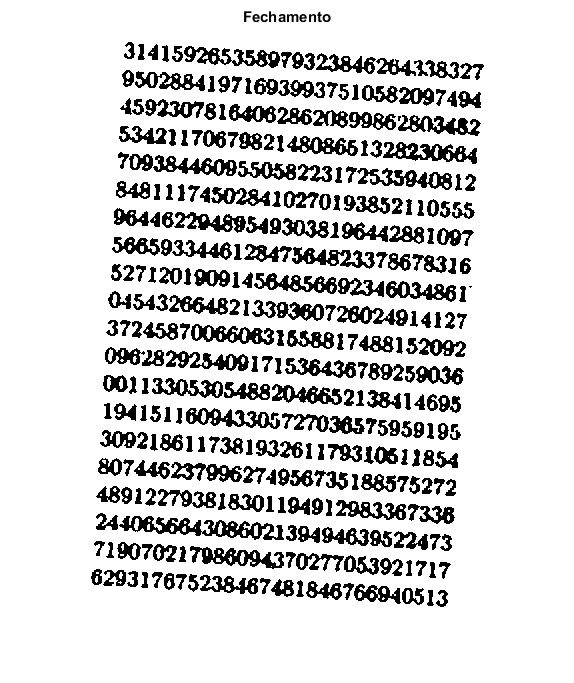
\includegraphics[scale=0.25]{fechamento.png}
	\caption{Resultado}
	\label{Original}
\end{figure}


\subsection{Parte II}

Na segunda parte, foram seguidos os passos solicitados e os resultados obtidos para tratar a imagem abaixo serão descritos a seguir

\begin{figure}[!htb]
	\centering
	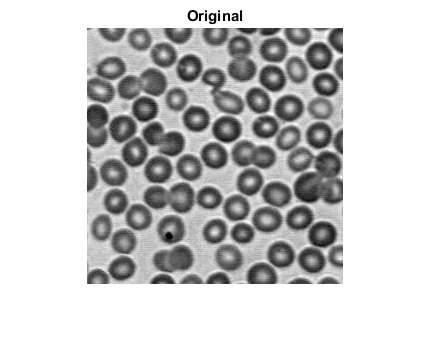
\includegraphics[scale=0.5]{2.png}
	\caption{Original}
	\label{Original}
\end{figure}

\subsubsection*{2.1}
A imagem foi binarizada como na primeira parte, onde as células são pretas e o fundo é branco

\begin{figure}[!htb]
	\centering
	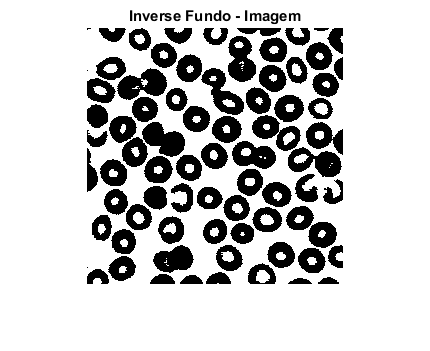
\includegraphics[scale=0.5]{2-1.png}
	\caption{Imagem binarizada}
	\label{Original}
\end{figure}

\subsubsection*{2.2}
A função \textit{bwareopen} para preencher espaços desconectados\newline
\\ 

\begin{figure}[!htb]
	\centering
	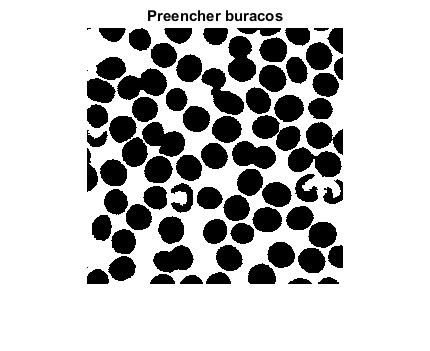
\includegraphics[scale=0.5]{2-buracos.png}
	\caption{Imagem Buracos Preenchidos}
	\label{Original}
\end{figure}

\subsubsection*{2.3}
A distância foi calculada através da função \textit{bwdist} usando o complemento da imagem

\begin{figure}[!htb]
	\centering
	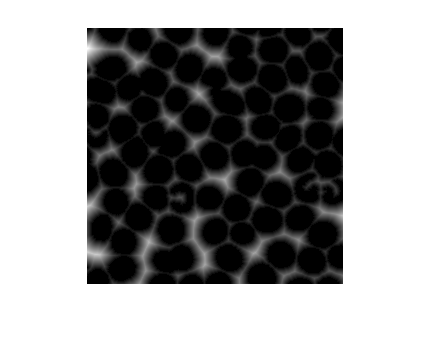
\includegraphics[scale=0.5]{2distancia.png}
	\caption{Distância}
	\label{Original}
\end{figure}

\subsubsection*{2.4}
Por fim, essa imagem foi segmentada, a fim de dividir os objetos que a compõe\newline
\\ 

\begin{figure}[!htb]
	\centering
	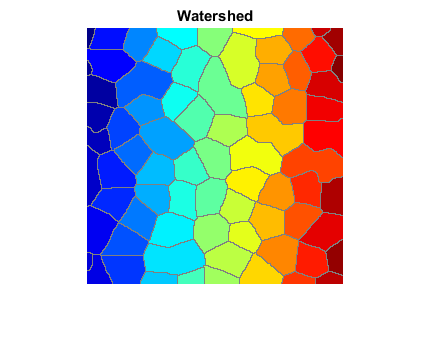
\includegraphics[scale=0.5]{2-wathershed.png}
	\caption{Distância}
	\label{Original}
\end{figure}

Nota-se que a imagem não foi perfeitamente segmentada, ou seja, os objetos não foram todos perfeitamente divididos, já que na binarização algumas células se mantiveram unidas, mesmo aplicando outras operações morfológicas para separá-las.

\subsection{Parte III}
Na terceira e última parte, foi feita uma função ler\_yuv que recebe como parâmetros um arquivo YUV, sua resolução, o formato (4:2:0) e o número do quadro a ser lido, e seu retorno é a imagem desse quadro.

A seguir são feitas novas funções que estimam o movimento (DPCM) entre um quadro e outro, recuperados a partir da função já citada. Essas funções foram feitas a partir do algoritmo de Block Matching para estimação de movimento.

As funções implementadas no projeto foram:

\begin{itemize}
	\item LogSearch;
	\item Motion\_Est;
	\item reconstruct;
	\item FullSearch;
	\item Bidirectional\_ME.
\end{itemize}

Resultados obtidos com blocos de tamanho 8x8 a partir dos frames 100 e 150 do arquivo '\textit{foreman.yuv}':

\begin{figure}[h]
\centering
\subfigure[Vetores de movimento]{
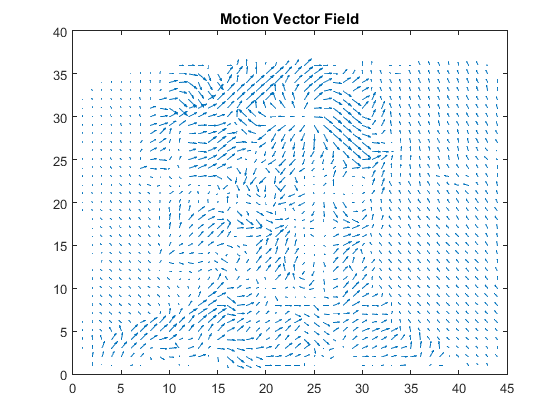
\includegraphics[scale=0.25]{3-1-motionvec.png}}
\subfigure[1º Frame]{
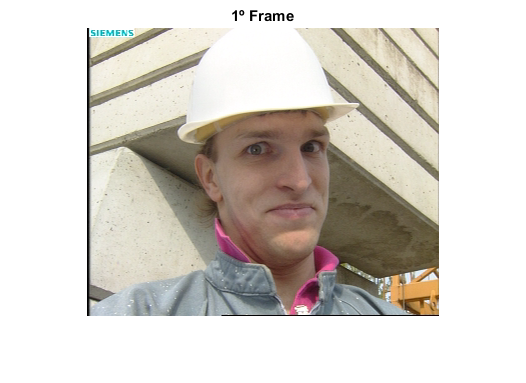
\includegraphics[scale=0.25]{3-1-f1.png}}
\subfigure[2º Frame\label{red2}]{
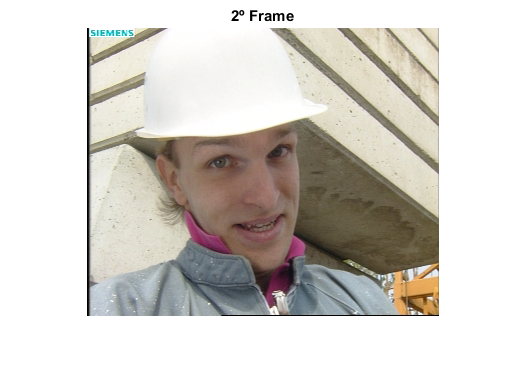
\includegraphics[scale=0.25]{3-1-f2.png}}
\subfigure[Resultado\label{red2}]{
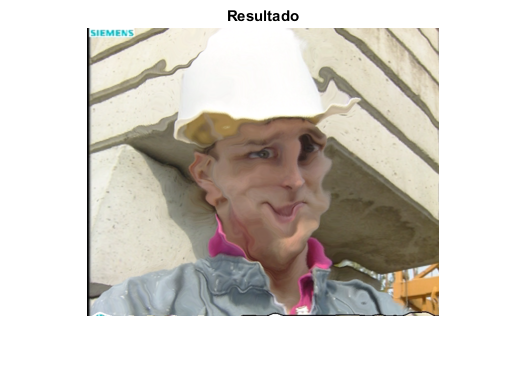
\includegraphics[scale=0.25]{3-1-resultado.png}}
\subfigure[SPRN]{
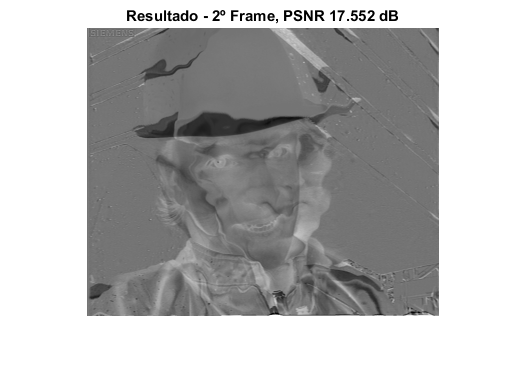
\includegraphics[scale=0.25]{3-1-psnr.png}}
\end{figure}

Resultados obtidos com blocos de tamanho 4x4 a partir dos frames 100 e 150 do arquivo '\textit{foreman.yuv}':

\begin{figure}[h]
\centering
\subfigure[Vetores de movimento]{
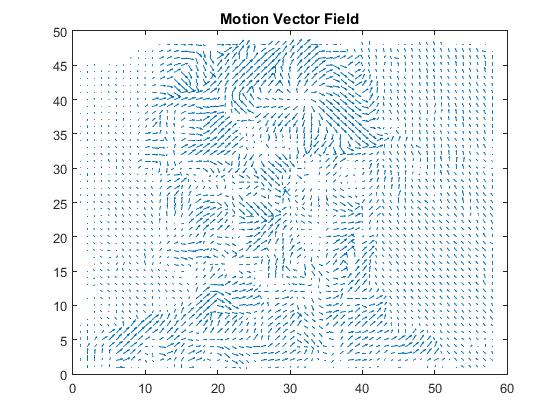
\includegraphics[scale=0.25]{3-2-motionvec.png}}
\subfigure[1º Frame]{
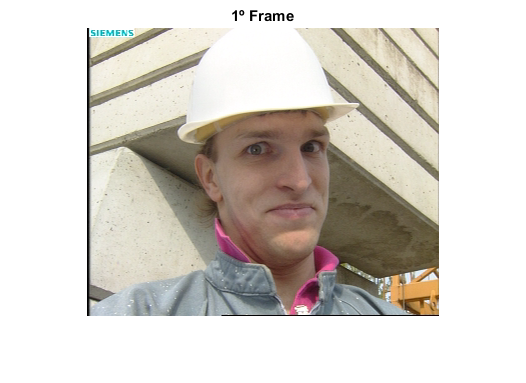
\includegraphics[scale=0.25]{3-2-f1.png}}
\subfigure[2º Frame\label{red2}]{
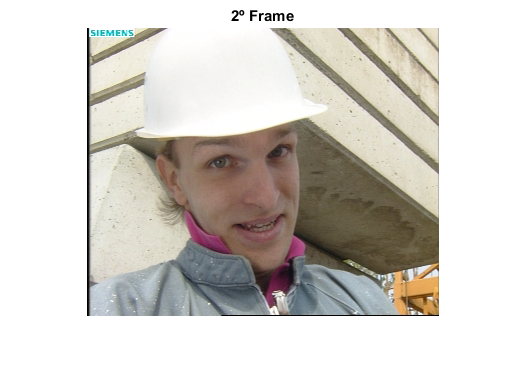
\includegraphics[scale=0.25]{3-2-f2.png}}
\subfigure[Resultado\label{red2}]{
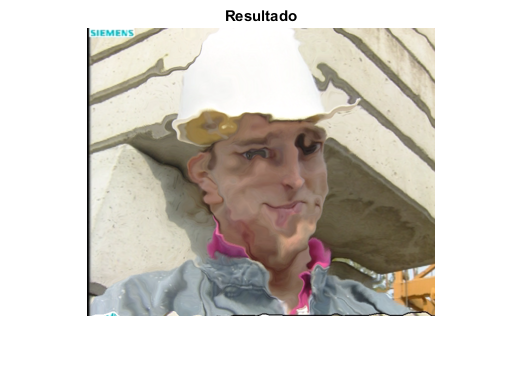
\includegraphics[scale=0.25]{3-2-resultado.png}}
\subfigure[SPRN]{
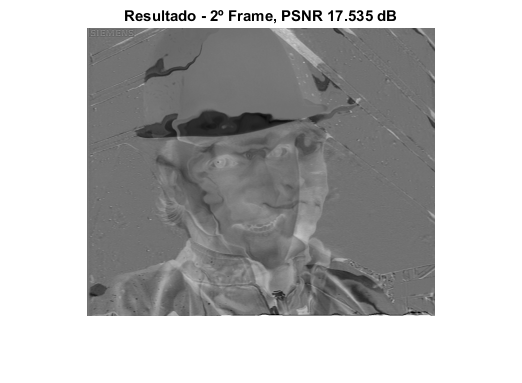
\includegraphics[scale=0.25]{3-2-psnr.png}}
\end{figure}

É notório como quanto menor o bloco, melhor a estimativa do movimento.

\ifCLASSOPTIONcaptionsoff
  \newpage
\fi

\section{Conclusão}
A partir dos resultados obtidos, na primeira parte nota-se que a definição da morfologia bottom-hat, que destaca objetos escuros sobre um fundo claro, aplicando fechamento na imagem para obter o fundo e posteriormente subtraindo a imagem por esse fundo encontrado é afirmada. Na segunda parte, aplicando segmentação seguindo os passos instruídos, tem-se o subdivisão da imagem em objetos ou regiões como era esperado, podendo servir para diversas aplicações que necessitam dos objetos isolados. E, por fim, um vídeo YUV é lido a partir dos parâmetros solicitados, e são recuperados frames especificos nessa função e aplica-se o algoritmo de Block Matching para estimação do movimento que foi claramente aplicado.

\begin{thebibliography}{1}

\bibitem{IEEEhowto:kopka}

http://scholar.harvard.edu/stanleychan/software/subpixel-motion-estimation-without-interpolation

Materiais da disciplina

\end{thebibliography}




\end{document}


